\newpage
\chapter{System Requirement Specification}

\section{Overall Description}

\subsection{Block Diagram}

\begin{figure}[H]
    \centering
    \includegraphics[width=1.0\linewidth]{image.png}
    \caption{SamaySetu System Block Diagram}
    \label{fig:block_diagram}
\end{figure}

The block diagram shown in Figure~\ref{fig:block_diagram} presents the overall architecture of the SamaySetu platform. The system is organised as a classic three-tier web application with a dedicated cache tier and an outbound email integration. The following subsections describe each tier and its constituent components.

\subsubsection{1. User Layer}

Four distinct user roles interact with the system, each through a role-appropriate interface rendered by the same underlying React application:

\begin{itemize}
    \item \textbf{Administrator} --- Full platform access. Manages all master data, approves new teachers, builds and publishes timetables for every division, and configures system-wide settings.
    \item \textbf{Head of Department (HOD)} --- Senior faculty role. Approves teachers in their department, manages academic structure, and builds timetables for divisions within their department.
    \item \textbf{Timetable Coordinator} --- Faculty volunteer role dedicated to schedule building. Has full timetable-building permissions but cannot manage staff accounts or approve teachers.
    \item \textbf{Teacher} --- Regular faculty member. Reads their own personal weekly published timetable, manages their profile, updates their weekly availability preferences, and changes their own password.
\end{itemize}

\subsubsection{2. Web Application (Frontend)}

The frontend is a React 18 single-page application written in TypeScript and built using Vite. It communicates with the backend exclusively through a REST API and uses JSON Web Tokens for authentication. Its main responsibilities are:

\begin{itemize}
    \item \textbf{Authentication flows} --- login, registration, email verification, forgot-password, reset-password, and first-login password change.
    \item \textbf{Role-aware routing} --- a single \texttt{ProtectedRoute} component gates every non-public route, redirecting unauthorised users to an appropriate home path.
    \item \textbf{Dashboards} --- separate dashboards for admin-layout roles (Admin, HOD, Timetable Coordinator) and for teachers, each presenting role-appropriate metrics and quick links.
    \item \textbf{Master-data CRUD pages} --- Academic Years, Departments, Courses, Divisions, Batches, Rooms, Time Slots, Staff.
    \item \textbf{Timetable builder} --- a visual grid with day columns and time-slot rows, supporting click-to-add, click-to-edit, drag-to-move, and drag-to-swap interactions.
    \item \textbf{Teacher views} --- personal weekly timetable, profile page, availability editor.
    \item \textbf{Export triggers} --- initiate PDF and Excel downloads through the backend export endpoints.
\end{itemize}

\subsubsection{3. Backend (Spring Boot REST API)}

The backend is a Spring Boot 3.5.5 application running on Java 17, packaged as a self-contained JAR with an embedded Tomcat web server on port 8083. Its responsibilities are divided across the following categories of components:

\textbf{Controllers} expose REST endpoints. The significant controllers are:
\begin{itemize}
    \item \texttt{AuthController} --- \texttt{/auth/login}, \texttt{/register}, \texttt{/verify-email}, \texttt{/forgot-password}, \texttt{/reset-password}, \texttt{/change-first-password}.
    \item \texttt{AdminController} --- CSV staff upload, manual staff creation, template downloads, bulk course upload.
    \item \texttt{AcademicController} --- CRUD for academic years.
    \item \texttt{DepartmentController}, \texttt{CourseController}, \texttt{DivisionController}, \texttt{BatchController}, \texttt{RoomController}, \texttt{TimeSlotController} --- CRUD for the respective academic entities.
    \item \texttt{TeacherController} --- teacher listing, approval queue, approve/reject.
    \item \texttt{StaffController} --- own-profile, own-password, own-availability endpoints.
    \item \texttt{TimetableController} --- the core of the system; entries CRUD, lab session creation, draft/publish/archive lifecycle, copy-from-division, pre-publish validation, and PDF/Excel export.
\end{itemize}

\textbf{Services} contain business logic:
\begin{itemize}
    \item \texttt{TeacherService} implements Spring Security's \texttt{UserDetailsService} and handles the full teacher lifecycle including registration, verification, approval, password management, and first-login flow.
    \item \texttt{AdminService} orchestrates CSV parsing and bulk staff creation.
    \item \texttt{TimetableService} handles the complete draft-edit-publish-archive lifecycle and integrates with the conflict checker before every write.
    \item \texttt{ConflictCheckService} implements the eight-point conflict detection engine described in Chapter 5.
    \item \texttt{TimetableValidationService} implements the pre-publish dashboard distinguishing blocking errors from informational warnings.
    \item \texttt{TimetableExportService} generates server-side PDFs via OpenPDF and Excel workbooks via Apache POI.
    \item \texttt{AuditLogService} emits structured \texttt{[AUDIT]} log entries for administrator-sensitive actions.
    \item \texttt{EmailService} dispatches verification, welcome, approval, rejection, and password-reset emails via Gmail SMTP.
    \item \texttt{AcademicService}, \texttt{DepartmentService}, \texttt{CourseService}, \texttt{DivisionService}, \texttt{RoomService}, \texttt{TimeSlotService} --- CRUD services for their respective entities.
\end{itemize}

\textbf{Repositories} are Spring Data JPA interfaces, one per entity. The \texttt{TimetableEntry\_repo} includes custom \texttt{@Query} methods for the conflict checks (\texttt{isTeacherBooked}, \texttt{isRoomBooked}, \texttt{isDivisionBooked}, \texttt{countTeacherPeriodsOnDay}, \texttt{calculateTeacherWeeklyMinutes}).

\textbf{Filters} execute before controller routing:
\begin{itemize}
    \item \texttt{RateLimitFilter} enforces per-IP sliding-window rate limits on authentication endpoints to defeat brute-force attacks.
    \item \texttt{JWTRequestFilter} extracts the \texttt{Authorization: Bearer} header, validates the token, loads the user via \texttt{TeacherService}, and sets the Spring Security context.
\end{itemize}

\textbf{Configuration} classes bootstrap cross-cutting concerns:
\begin{itemize}
    \item \texttt{SecurityConfig} declares the Spring Security filter chain, CORS policy, URL-level access rules, structured 401 and 403 response handlers, and the \texttt{AuthenticationManager} bean.
    \item \texttt{RedisConfig} configures the Redis cache manager with a custom serializer that correctly handles \texttt{java.sql.Timestamp}.
    \item \texttt{InputSanitizationAdvice} is a \texttt{@RestControllerAdvice} that sanitises String fields in request bodies to neutralise XSS payloads.
\end{itemize}

\subsubsection{4. Data Layer}

The persistence tier consists of two cooperating stores:

\begin{itemize}
    \item \textbf{PostgreSQL 17} --- primary relational database. Stores all master data and all timetable entries across their complete DRAFT / PUBLISHED / ARCHIVED lifecycle. Hibernate's \texttt{ddl-auto=update} manages schema in development; production uses \texttt{validate} with migrations.
    \item \textbf{Redis} --- read-path cache for published timetables. Spring's \texttt{@Cacheable} annotations on \texttt{TimetableService.getDivisionTimetable()} and \texttt{getTeacherTimetable()} transparently serve from cache; \texttt{@CacheEvict} annotations on the publish, archive, and update paths keep the cache consistent.
\end{itemize}

\subsubsection{5. Output and Export Module}

The timetable view builder renders three orthogonal views from the same underlying data:
\begin{itemize}
    \item \textbf{Division-wise timetable} --- standard weekly grid for a division.
    \item \textbf{Teacher-wise timetable} --- a teacher's personal view across all their divisions.
    \item \textbf{Room-wise view} (read-only, derived from the timetable entries) --- shows classroom and laboratory utilisation.
\end{itemize}

Server-side export:
\begin{itemize}
    \item \textbf{OpenPDF} --- produces A4 landscape PDF exports with institutional branding, merged break rows, and colour-coded laboratory cells.
    \item \textbf{Apache POI} --- produces \texttt{.xlsx} Excel workbooks with equivalent styling.
\end{itemize}

\subsubsection{6. External Integrations}

\begin{itemize}
    \item \textbf{Gmail SMTP} --- outbound email delivery for verification, welcome, approval, rejection, and password-reset messages.
    \item \textbf{AWS} --- production deployment target: EC2 with ALB for the backend, RDS for PostgreSQL, ElastiCache for Redis, and Amplify for the frontend.
    \item \textbf{GitHub Actions} --- continuous integration on every push; manual workflow-dispatch trigger for AWS deployment.
\end{itemize}

\subsubsection{7. Overall Working Flow}

\begin{enumerate}
    \item The administrator logs in. Authentication is verified against the \texttt{users} table and a JWT is returned to the browser.
    \item The administrator incrementally enters master data (academic year, departments, courses, divisions, rooms, time slots, staff). Each CRUD call is gated by role-based authorisation.
    \item The administrator opens the Timetable Builder, selects an academic year and a division, and sees an empty or partially-filled grid.
    \item The administrator adds, edits, moves, or swaps entries using clicks and drag-drop gestures. Each write operation invokes the conflict engine, which either accepts the change or returns all detected conflicts.
    \item For laboratory sessions, the administrator uses the Lab Session Wizard, which atomically creates parallel batch entries linked through a shared lab session group.
    \item When ready, the administrator triggers pre-publish validation. Blocking errors must be resolved; warnings can be acknowledged.
    \item On publishing, the service archives any previously-published version, flips draft entries to PUBLISHED, and evicts the Redis caches.
    \item Teachers see the new published timetable; exports can be downloaded on demand; audit log entries record the publication event.
\end{enumerate}

\subsection{Sequence Diagram}

\begin{figure}[H]
    \centering
    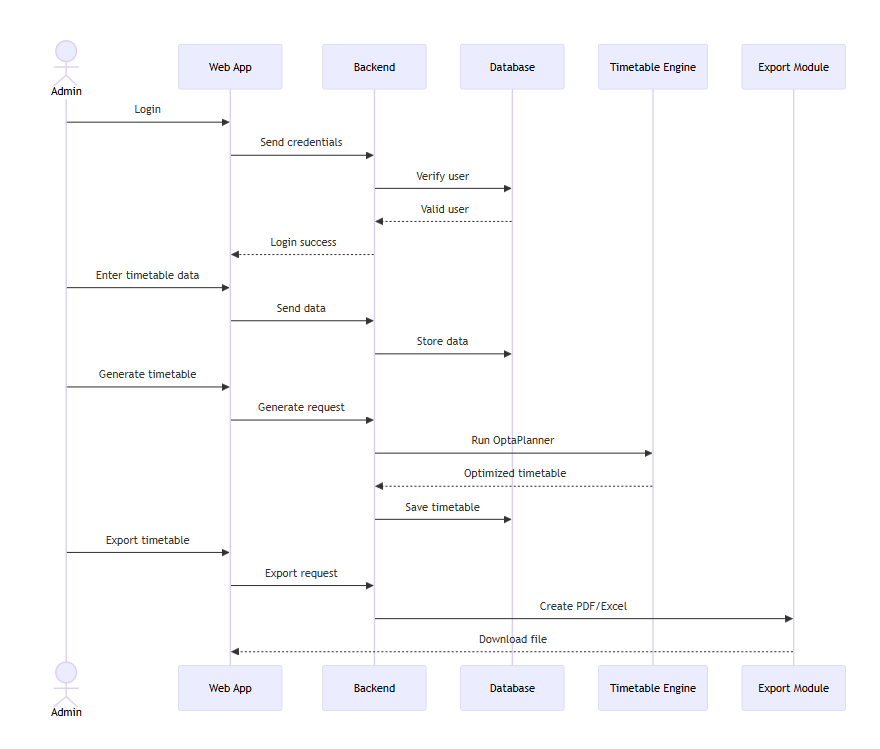
\includegraphics[width=1.0\linewidth]{image2.png}
    \caption{SamaySetu Sequence Diagram}
    \label{fig:seq_diagram}
\end{figure}

Figure~\ref{fig:seq_diagram} captures the four representative interactions between the Administrator, the Web Application (React), the Backend (Spring Boot), the Database (PostgreSQL), the Conflict and Validation Engine, and the Export Module.

\subsubsection{1. Login Process}

\begin{itemize}
    \item The administrator submits login credentials to the Web Application.
    \item The Web Application forwards them to \texttt{POST /auth/login} on the backend.
    \item The backend loads the user via \texttt{TeacherService.loadUserByUsername} from PostgreSQL, verifies the BCrypt-hashed password, checks that the account is active, verified, and approved, and --- on success --- returns a JWT along with the user's role and first-login flag.
    \item The Web Application persists the JWT to \texttt{localStorage} or \texttt{sessionStorage} (depending on the user's ``remember me'' choice) and routes the user to their role-specific home.
\end{itemize}

\subsubsection{2. Entering Timetable Data}

\begin{itemize}
    \item Once logged in, the administrator enters master data through the relevant CRUD interfaces.
    \item Each CRUD operation triggers a REST call (e.g.\ \texttt{POST /admin/api/courses}) carrying the \texttt{Authorization: Bearer} header.
    \item The backend's filter chain validates the JWT, Spring Security enforces role-based authorisation, the controller delegates to the corresponding service, the service invokes its JPA repository, and PostgreSQL persists the record.
    \item A JSON response is returned; the UI updates optimistically.
\end{itemize}

\subsubsection{3. Timetable Construction}

\begin{itemize}
    \item The administrator opens the Timetable Builder. The Web Application issues \texttt{GET /api/timetable/draft?divisionId=…\&academicYearId=…} to load the current draft.
    \item For each add / edit / drag-drop event, the Web Application calls \texttt{POST /api/timetable/entries} or \texttt{PUT /api/timetable/entries/\{id\}}.
    \item The \texttt{TimetableService} constructs a \texttt{TimetableEntryRequest} and invokes \texttt{ConflictCheckService.checkConflicts}. If no conflicts are found, the entry is saved and the UI reflects the change. If conflicts are found, the backend returns HTTP 409 with a structured list of human-readable messages, which the UI presents as a dismissable error panel.
    \item For laboratory sessions, the administrator invokes \texttt{POST /api/timetable/lab-session} through the Lab Session Wizard. The service creates the parent \texttt{LabSessionGroup} and $2 \times N$ child entries within a single database transaction.
\end{itemize}

\subsubsection{4. Publish and Export}

\begin{itemize}
    \item The administrator triggers \texttt{GET /api/timetable/validate?divisionId=…} to run pre-publish validation. The \texttt{TimetableValidationService} returns a structured result listing errors and warnings.
    \item If the result is acceptable, the administrator calls \texttt{POST /api/timetable/publish?divisionId=…\&academicYearId=…}. The service archives any currently-published entries for the same division + year, flips draft entries to PUBLISHED, and evicts Redis caches.
    \item For export, the administrator calls \texttt{GET /api/timetable/export/division/\{id\}/pdf} (or \texttt{/excel}). The \texttt{TimetableExportService} generates the file in-memory and streams it back as a download.
\end{itemize}

\section{Project Planning}

\begin{figure}[H]
    \centering
    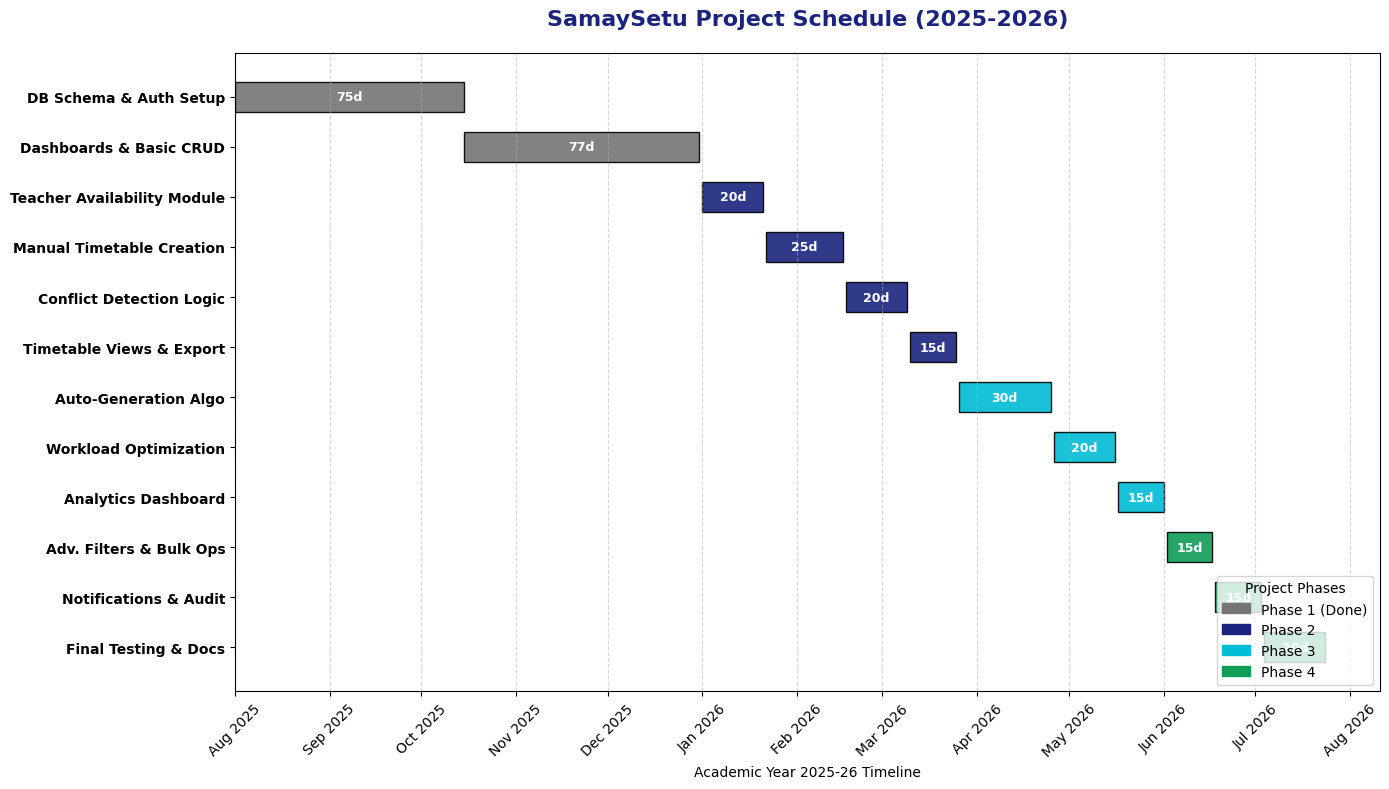
\includegraphics[width=1.0\linewidth]{planning.png}
    \caption{Project Planning Timeline (Academic Year 2025--2026)}
    \label{fig:project_plan}
\end{figure}

The project was executed across the academic year 2025--2026 in four logical phases, each with clearly-defined deliverables.

\subsubsection{Phase 1: Foundation and Core Infrastructure (August 2025 -- October 2025)}

The first phase established the systemic backbone of the platform.
\begin{itemize}
    \item \textbf{Database schema and authentication setup (approximately 75 days)} --- Designed all relational tables, set up Hibernate-managed schema, implemented JWT-based authentication with Spring Security, added BCrypt password hashing, and built the login, registration, email verification, forgot-password, and first-login flows.
    \item \textbf{Dashboards and basic master-data CRUD (approximately 77 days)} --- Developed the administrator and teacher dashboards along with CRUD interfaces for academic years, departments, courses, rooms, divisions, batches, time slots, and staff.
\end{itemize}
\textit{Outcome:} A secure, authenticated, multi-role web application capable of managing the institution's master data.

\subsubsection{Phase 2: Timetable Builder and Conflict Prevention (November 2025 -- March 2026)}

The second phase delivered the core scheduling functionality.
\begin{itemize}
    \item \textbf{Teacher availability module} --- Allowed teachers to record per-slot availability preferences.
    \item \textbf{Manual timetable grid} --- Implemented the day-column, time-slot-row grid with click-to-add and click-to-edit interactions.
    \item \textbf{Conflict detection engine} --- Implemented the eight-point rule set covering break protection, teacher, room, division, daily period limit, weekly hour limit, room capacity, and room-course type.
    \item \textbf{Drag-and-drop} --- Added accessible drag-to-move and drag-to-swap interactions using dnd-kit.
    \item \textbf{Lab Session Wizard} --- Atomic creation of parallel batch entries linked through a lab session group.
    \item \textbf{Export module} --- Server-side PDF (OpenPDF) and Excel (Apache POI) generation for both division and teacher views.
    \item \textbf{Pre-publish validation and lifecycle} --- Blocking/warning validation dashboard, publish workflow with automatic archival of previous versions, and Redis cache eviction.
\end{itemize}
\textit{Outcome:} A fully-functional timetable-management system end-to-end.

\subsubsection{Phase 3: Hardening and Security (April 2026 -- May 2026)}

The third phase focused on making the system production-ready.
\begin{itemize}
    \item \textbf{Rate limiting} on authentication endpoints to defeat brute-force attacks.
    \item \textbf{Input sanitisation} on all request bodies as a defence-in-depth against cross-site scripting.
    \item \textbf{Audit logging} of administrator-sensitive actions in a structured \texttt{[AUDIT]} format.
    \item \textbf{Security headers} --- HSTS, X-Frame-Options, Content-Security-Policy, Cache-Control.
    \item \textbf{Structured 401 / 403 responses} enabling the frontend to distinguish auth failures from validation failures.
    \item \textbf{Redis serializer hardening} for correct \texttt{Timestamp} round-trips.
    \item \textbf{Environment-driven configuration} with complete separation of development and production profiles.
\end{itemize}
\textit{Outcome:} A hardened system suitable for institutional deployment.

\subsubsection{Phase 4: Deployment and Documentation (June 2026 -- July 2026)}

The final phase focused on delivery.
\begin{itemize}
    \item \textbf{AWS deployment scripts} for EC2 Auto Scaling Group, ALB, RDS PostgreSQL, and Amplify frontend.
    \item \textbf{GitHub Actions CI} and a manual deploy workflow.
    \item \textbf{End-to-end testing} across every role and every major user story.
    \item \textbf{Seed-data scripts} for realistic development and demonstration data.
    \item \textbf{Comprehensive project documentation}, including this report and a developer-focused project bible.
\end{itemize}
\textit{Outcome:} A stable, documented, deployable release.

\subsection{Overall Summary}

The four-phase plan provided:
\begin{itemize}
    \item \textbf{Progressive development} from foundational infrastructure to advanced features.
    \item \textbf{Clear separation of responsibilities} across phases, each with a specific set of deliverables.
    \item \textbf{Adequate buffer time} for iterative testing and security hardening.
    \item \textbf{A stable, documented, deployment-ready final product} delivered within the academic year.
\end{itemize}

\vspace{10mm}
\hrule
